\documentclass[british]{ntnureport}

\title{An NTNU Report \LaTeX{} Document Class}
\shorttitle{An NTNU Report Document Class}
\author{Anders Kjelsrud \\
        Casper F. Gulbrandsen \\
		Kristian Jegerud \\ 
		Norges Teknisk-Naturvitenskapelige Universitet }
\shortauthor{CoPCSE$@$NTNU}
\date{CC-BY \ntnureportdate}

\addbibresource{report.bib}

\begin{document}

\begin{abstract}
    Emnet IMT3881 Vitenskapelig Programmering kombinerer realfaglige teknikker og høynivå programmering, og 
    gir studentene et innblikk i hvordan dette kan benyttes til å løse hverdagslige problemsstillinger. Et godt 
    eksempel på dette er bildebehandling, hvor numeriske løsninger av differensiallikninger og ikkelineære algebraiske
    likninger sammen med biblioteker fra Python kan benyttes til å behandle bilder. Hovedoppgaven vår har vært å
    implementere ulike anvendelser for dette, både for fargebilder og gråtonebilder. Vi har også skrevet et lite
    program med grafisk brukergrensesnitt (GUI) som viser eksempler på anvendelsene vi har implemntert. Ved å lese
    denne rapporten får du innsikt i hvordan vi har jobbet, hvilke teknikker som er brukt og hvordan disse er
    benyttet. All kildekoden ligger tilgjengelig på GitLab\cite{gitsource}. 
\end{abstract}

\section{Introduksjon}

\subsection{Forrord}
Prosjektgruppen består av tre studenter fra dataingeniørstudiet ved NTNU Gjøvik. I løpet av 
semesteret har vi introdusert for matematiske teknikker for numeriske løsninger av bestemte 
integral, ordinære og systemer av differensiallikninger og ikkelineære algebraiske likninger. 
Vi har også fått lære om høynivå programmering for lineæralgebra, optimalisering, bildebehandling 
og maskinlæring. Oppgaven som ble gitt innebærte at vi måtte benytte oss av de vi har lært i løpet
av semesteret. Selv om det har vært masse utfordringer underveis har vi fått masse praktisk 
læring. 

\subsection{Oppgavedefinisjon}

\subsection{Gruppens deltagere}
Gruppen vår består av tre studenter på dataingeniørstudiet ved NTNU Gjøvik. Siden de to første årene på
studiet utelukkende består av obligatoriske fag, har vi stort sett de samme kunnskapene og 
forutsetningene før prosjektets start. Uansett gjør det at vi er en gruppe på 3 at vi møter utfordringer
med ulike tilnærminger, og har vært viktig for å løse problemstillingene på en best mulig måte.

Vi har ikke benyttet Python som hovedprogrammeringsspråk i emner vi har deltatt i før dette semesteret,
men har før prosjektets start benyttet det i alle arbeidskrav i emnet. Dette gjør at vi har en viss 
kjennskap til hvordan Python fungerer og hvilke fordeler og ulemper dette medfører. For oss har nok den 
største utfordringer med Python vært hvordan vi skal strukturere et såpass stort prosjekt med flere 
forskjellige filtyper. Ingen av oss har vært borti utvikling av en GUI-applikasjon med Python og Qt som 
programmeringsspråk før. Dette har derfor gitt en bratt læringskurve og masse læring.

Rapporten er skrevet med LaTeX, som er et språk vi har brukt på et mindre prosjekt tidligere på studiet.
Når vi har skrevet rapporten har det ikke gitt oss noen nevneverdige utfordringer. Det har derimot gitt
oss utfordringer når rapporten måtte holdes lagret sammen med kildekoden i GitLab. Særlig når vi skulle
finne en god editor for å jobbe på de ulike rapportfilene samtidig slet vi med å finne en løsning som 
vi synes var effektiv.


\section{Using the Document Class}
\label{chap:usage}

\subsection{Report Setup and Language Selection}
\label{sec:setup}

The document class is initialized by issuing the \texttt{\textbackslash documentclass[]\{ntnureport\}} at the beginning of your \texttt{.tex} file. The report language should be given as an option. Currently British English (class option \texttt{[british]}), American English (class option \texttt{[american]}), Norwegian Bokmål (class option \texttt{[norsk]}) and Norwegian Nynorsk (class option \texttt{[nynorsk]}) are supported.\footnote{Disclaimer: this unfortunate naming of the Norwegian language options follows from the naming conventions of the \texttt{babel} package.}

\subsection{Title, Author, and Date}

In the preample of the \texttt{.tex} file, the report title should be set with the \texttt{\textbackslash title\{\}} command. The title will appear on the titlepage as well as in the running header of the even numbered pages. If the title is too long for the header, you can use \texttt{\textbackslash shorttitle\{\}} to set a version for the header.

The authors should be listed with full names in the \texttt{\textbackslash author\{\}} command. If there are several authors, they should be separated with \texttt{\textbackslash and}, e.g., like this: \texttt{\textbackslash author\{Anne Andersen \textbackslash and Bjørn Bjørnsen\}}. For the running headers, you may want to use \texttt{\textbackslash shortauthor}, e.g. like this: \texttt{\textbackslash shortauthor\{A. Andersen and B. Bjørnsen\}} or even \texttt{\textbackslash shortauthor\{Andersen et al.\}}.

Use \texttt{\textbackslash date\{\}} to set the date of the document. To keep track of temporary versions, it can be a good idea to use \texttt{\textbackslash date\{\textbackslash today\}} while working on the report. You may also add copyright and licence information in this field.

\subsection{Page Layout}

The document class is designed to work with twosided printing. However, since the theses are very often read on displays, the margins are kept the same on even and odd pages in order to avoid that the page is jumping back and forth upon reading.

\subsection{Structuring Elements}

The standard \LaTeX{} elements for document structure are supported: section, subsection, and:

\subsubsection{This is a \texttt{\textbackslash subsection\{\}}}

Short subsubsection text here.

\paragraph{This is a \texttt{\textbackslash paragraph\{\}}}

Short paragraph text here.

Don't use too many levels of headings; how many are appropriate, will depend on the size of the document. Also, don't use headings too frequently.

Make sure that the chapter and section headings are correctly capitalised depending on the language of the report, e.g., `\emph{Correct Capitalisation of Titles in English}' vs. `\emph{Korrekt staving av titler på norsk}'. 

Simple paragraphs are the lowest structuring elements and should be used the most. They are made by leaving one (or more) blank line(s) in the \texttt{.tex} file. In the typeset document they will appear indented with no vertical space between them.

\subsection{Lists}

Numbered and unnumbered lists, i.e., the \texttt{enumerate} and \texttt{itemize} environments, are used just as in regular \LaTeX{}, but are typeset somewhat more densely and with other labels. Unnumbered list:
\begin{itemize}
    \item first item
    \item second item
    \begin{itemize}
        \item first subitem
        \item second subitem
        \begin{itemize}
            \item first subsubitem
            \item second subsubitem
        \end{itemize}
    \end{itemize}
    \item last item
\end{itemize}
Numbered list:
\begin{enumerate}
    \item first item
    \item second item
    \begin{enumerate}
        \item first subitem
        \item second subitem
        \begin{enumerate}
            \item first subsubitem
            \item second subsubitem
        \end{enumerate}
    \end{enumerate}
    \item last item
\end{enumerate}

For description lists, see usage in, e.g., \cref{sec:frontmatter}.

\subsection{Figures}

Figures are placed in the \texttt{figure} environment. An example is shown in \cref{fig:mapNTNU}. Figures are floats, hence they will float freely around in the document in accordance with standard \LaTeX{} behaviour. You may want to try to override \LaTeX{}'s default placement by using the \texttt{h} (here), \texttt{t} (top of page), \texttt{b} (bottom of page), and \texttt{p} (separate page) options in order of priority. If you provide an alternate (typically shorter) caption in square brackets, it will be used in the list of figures. Use \texttt{\textbackslash includegraphics[]\{\}} with options \texttt{scale} or \texttt{width} to include the graphics file. The caption should be placed \emph{below} the figure. If the caption consists of a single sentence fragment (incomplete sentence), it should not be punctuated. Given the shape and size of the figure, the figure caption can appear too close or too far from the figure. To deal with this, vertical space, either positive or negative, can be added before and/or after the caption command using the \texttt{\textbackslash vspace{}} command.

\begin{figure}[htbp]  % order of priority: h here, t top, b bottom, p page
  \centering
  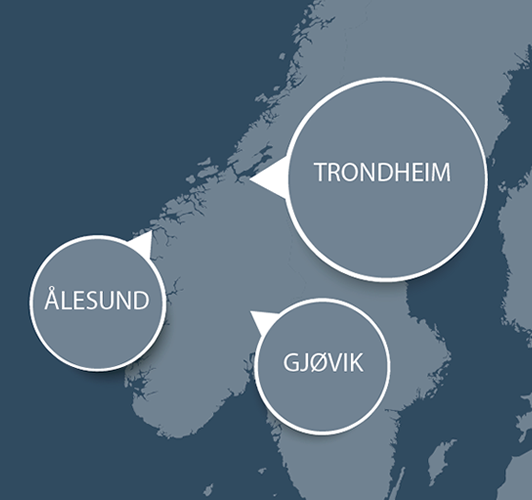
\includegraphics[width=.5\textwidth]{figures/kart_student}
  \caption[Map of NTNU Campuses]{The map shows the three main campuses of NTNU.}
  \label{fig:mapNTNU}
\end{figure}

For figures compsed of several sub-figures, the \texttt{caption} and \texttt{subcaption} packages have been preloaded. See \cref{fig:subfig} with \cref{sfig:a,sfig:b} for an example. For more details on alignment etc., see the Overleaf documentation.\footnote{\url{https://www.overleaf.com/learn/latex/How_to_Write_a_Thesis_in_LaTeX_(Part_3):_Figures,_Subfigures_and_Tables}}

\begin{figure}
    \centering
    \begin{subfigure}[b]{.45\textwidth}
        \centering
        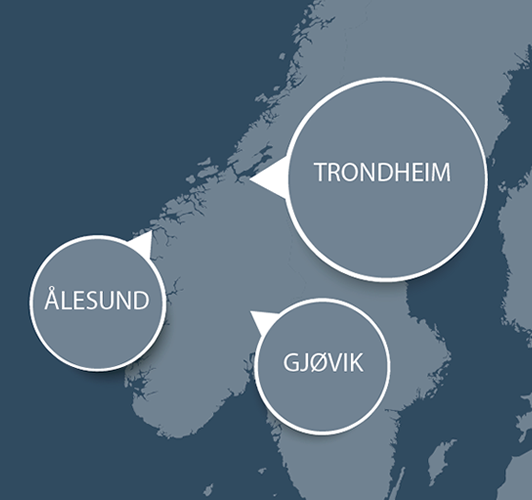
\includegraphics[width=\textwidth]{figures/kart_student.png}
        \caption{First sub-figure}
        \label{sfig:a}
    \end{subfigure}
    \hfill
    \begin{subfigure}[b]{.45\textwidth}
        \centering
        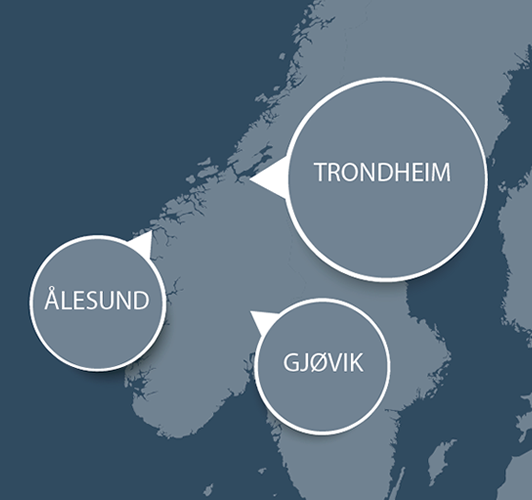
\includegraphics[width=\textwidth]{figures/kart_student.png}
        \caption{Second sub-figure}
        \label{sfig:b}
    \end{subfigure}
    \caption{A figure composed of two sub-figures. It has a long caption in order to demonstrate how that is typeset.}
    \label{fig:subfig}
\end{figure}

\subsection{Tables}

Tables are placed in the \texttt{table} environment. An example is given in \cref{tab:example1}. Like figures, tables float freely around in the document in accordance with standard \LaTeX{} behaviour. The table caption should be placed \emph{above} the table. If the caption consists of a single sentence fragment (incomplete sentence), it should not be punctuated.

\begin{table}
  \centering
  \caption{A simple, manually formatted example table}
  \label{tab:example1}
  \begin{tabular}{cc}
    \hline
    age  & IQ \\ 
    \hline
    10   & 110 \\
    20   & 120 \\
    30   & 145 \\
    40   & 120 \\
    50   & 100 \\
    \hline
  \end{tabular}
\end{table}

Tables can also be automatically generated from CSV files using the \texttt{simplecsv} and \texttt{booktab} packages. See \cref{tab:examplecsv} for an example.

\begin{table}[tbp]
  \centering
  \caption[A simple example table generated from a CSV file]{A simple example table generated from a CSV file using \texttt{simplecsv} and \texttt{booktab}}
  \label{tab:examplecsv}
  \csvautobooktabular{csvtables/ageiq.csv}
\end{table}

\subsection{Listings}

Code listings are included by means of the \texttt{listings} package. Code examples can be read from file or provided inline, and should be given a caption for cross referencing and for appearance in the list of code listings in the report frontmatter. If all your code examples are written in the same programming language, you can use, e.g., \texttt{\textbackslash lstset\{language=Python\}} to set the language once and for all. The code is set with the monospace font, and the font size is reduced to allow for code lines up to at least 80 characters without causing line breaks. Options for programming languages, line numbering etc. are provided. Unlike figures and tables, code listings are not floating objects, and will appear at the same position in the typeset document as in the \texttt{.tex} file. If the caption consists of a single sentence fragment (incomplete sentence), it should not be punctuated.

\lstinputlisting[
    caption={Python example from file},
    label=lst:pythonfile,
    language=Python
]{listings/example.py}

\lstinputlisting[%
    caption={C++ example from file},
    label=lst:cppfile,
    language=C++,
    numbers=left
]{listings/example.cc}

\begin{lstlisting}[
    caption={Python code in \LaTeX{} document},
    label=lst:pythondoc,
    language=Python]
import numpy as np
import matplotlib.pyplot as plt

x = np.linspace(0, 1)
y = np.sin(2 * np.pi * x)

plt.plot(x, y)
plt.show()
\end{lstlisting}

\begin{lstlisting}[
    caption={C++ code in \LaTeX{} document},
    label=lst:cppdoc,
    language=C++]
#include <iostream>
using namespace std;

int main() 
{
  cout << "Hello, World!" << endl;
  return 0;
}
\end{lstlisting}

\subsection{Equations}

Equations are typeset as normally in \LaTeX{}. It is common to consider equations part of the surrounding sentences, and include punctuation in the equations accordingly, e.g.,
\begin{equation}
    f(x) = \int_1^x \frac{1}{y}\,dy = \ln x\,.
    \label{eq:logarithm}
\end{equation}
For more advanced symbols like, e.g., $\mathbb{R}, \mathbb{Q}$, the \texttt{amssymb} package is preloaded, and for more advanced mathematical layout the \texttt{amsmath} behaviour is obtained through the \texttt{mathdesign} package. Confer the Overleaf documentation for details.\footnote{\url{https://www.overleaf.com/learn/latex/Mathematical_expressions}}

\subsection{Fonts}

Bitstream Charter at 11pt with the corresponding Mathdesign math fonts have been selected as the main fonts for the report template. For code examples, the monospaced font should be used – for this, a scaled version of the DejaVuSansMono to match the main font is preselected. If you would like to use an accompanying sans serif font, the BeraSans has been made available. The standard \LaTeX{} font commands should be used to switch between fonts, e.g.,
\texttt{\textbackslash textit\{\}} \textit{for italics},
\texttt{\textbackslash textbf\{\}} \textbf{for bold face},
\texttt{\textbackslash texttt\{\}} \texttt{for mono spaced}, and
\texttt{\textbackslash textsf\{\}} \textsf{for sans serif}.
For generic \emph{emphasis}, \texttt{\textbackslash emph\{\}} should be applied.

\subsection{Cross References}
\label{sec:crossref}

For cross references, i.e., references within the document, the \texttt{\textbackslash cref\{\}} command provided byt the \texttt{cleveref} package should be used. Labels are inserted in the document in the standard \LaTeX{} manner. They are case sensitive, so, e.g., a label immediately after a section command refers to that section, while a label within, e.g., a table environment refers to the table. The \texttt{\textbackslash cref\{\}} command also generates the corresponding text. If the document is in English (class options \texttt{british} or \texttt{american}), the cross references are capitalised, whereas if it is in Norwegian (class options \texttt{norsk} or \texttt{nynorsk}), they are not. If you are writing in Norwegian, you should use \texttt{\textbackslash Cref\{\}} at the beginning of a sentence to ensure that the cross reference is correctly capitalised. For examples on usage, see \cref{sec:crossref} in \cref{chap:usage}, \cref{tab:example1}, \cref{fig:mapNTNU}, \cref{eq:logarithm}, \cref{lst:cppfile}, and \cref{app:additional}. \Cref{app:additional} at the beginning of a sentence.

The cross references are made into active hyperlinks in the resulting PDF document by the use of the \texttt{hyperref} package. The colour of the links is set to black for best appearance on print. This can easily be changed by the author by the use of the \texttt{\textbackslash hypersetup\{\}} command.

\subsection{Bibliography}

The bibliography is typset using the \texttt{biblatex} package with the \texttt{biber} backend. The default citation style is \texttt{numeric-comp}, and the default bibliography style is \texttt{ieee}. This produces a bibliography similar to, but not completely according to, the so-called Vancouver style. With this setup, a single \texttt{\textbackslash cite\{\}} command will give a number only~\cite{landes1951scrutiny}, and \texttt{\textbackslash textcite\{\}} will give author and number like this: \textcite{landes1951scrutiny}. If you would like to give the full reference of a paper within the report, use \texttt{\textbackslash fullcite\{\}} like this: \fullcite{landes1951scrutiny}.

\subsection{Appendices}

Additional material that does not fit in the main report but may still be relevant to share, e.g., raw data from experiments and surveys, code listings, additional plots, pre-project reports, project agreements, contracts, logs etc., can be put in appendices. Simply issue the command \texttt{\textbackslash appendix} in the main \texttt{.tex} file, and then the following chapters made by \texttt{\textbackslash section\{\}} become appendices. See \cref{app:additional} for an example.
\section{Report Structure}

The structure of the report, i.e., which chapters and other document elements that should be included, depends on the type of project it describes (development, research, investigation, consulting), and the diversity (narrow, broad). Thus, there are no exact rules for how to do it, so whatever follows should be taken as guidelines only.

A report, like a book, can typically be divided into three parts: front matter, body matter, and back matter. Of these, the body matter is by far the most important one, and also the one that varies the most between report types.


\label{sec:frontmatter}

The front matter is everything that comes before the main part of the report. It is common to use roman page numbers for this part to indicate this. The minimum required front matter consists of a title page and an abstract:

\begin{description}
    \item[Title:] The title should, at minimum, include the report title, authors and a date.
    \item[Abstract:] The abstract should be an extremely condensed version of the report. Think one sentence with the main message from each of the chapters of the body matter as a starting point. \textcite{landes1951scrutiny} have given some very nice instructions on how to write a good abstract.
\end{description}

\subsection{Body Matter}

The body matter consists of the main chapters of the report. There is a great diversity in the structure chosen for different report types. Common to almost all is that the first chapter is an introduction, and that the last one is a conclusion followed by the bibliography.

\subsubsection{Development Project}
\label{sec:development}

For development projects, the main task is to develop something, typically a software prototype, for an `employer' (e.g., an external company or a research group). A report describing such a project is typically structured as a software development report with more or less the following chapters:

\begin{description}
    \item[Introduction:] The introduction of the report should take the reader all the way from the big picture and context of the project to the concrete task that has been solved in the report. A nice skeleton for a good introduction was given by \textcite{claerbout1991scrutiny}: \emph{review–claim–agenda}. In the review part, the background of the project is covered. This leads up to your claim, which is typically that some entity (software, device) or knowledge (research questions) is missing and sorely needed. The agenda part briefly summarises how your report contributes.
    \item[Requirements:] The requirements chapter should lead up to a concrete description of both the functional and non-functional requirements for whatever is to be developed at both a high level (use cases) and lower levels (low level use cases, requirements). If a classical waterfall development process is followed, this chapter is the product of the requirement phase. If a more agile model like, e.g., SCRUM is followed, the requirements will appear through the project as, e.g., the user stories developed in the sprint planning meetings.
    \item[Technical design:] The technical design chapter describes the big picture of the chosen solution. For a software development project, this would typically contain the system arcitechture (client-server, cloud, databases, networking, services etc.); both how it was solved, and, more importantly, why this architecture was chosen.
    \item[Development Process:] In this chapter, you should describe the process that was followed. It should cover the process model, why it was chosen, and how it was implemented, including tools for project management, documentation etc. Depending on how you write the other chapters, there may be good reasons to place this chapters somewhere else in the report.
    \item[Implementation:] Here you should describe the more technical details of the solution. Which tools were used (programming languages, libraries, IDEs, APIs, frameworks, etc.). It is a good idea to give some code examples. If class diagrams, database models etc. were not presented in the technical design chapter, they can be included here.
    \item[Deployment:] This chapter should describe how your solution can be deployed on the employer's system. It should include technical details on how to set it up, as well as discussions on choices made concerning scalability, maintenance, etc.
    \item[Testing and user feedback:] This chapter should describe how the system was tested during and after development. This would cover everything from unit testing to user testing; black-box vs. white-box; how it was done, what was learned from the testing, and what impact it had on the product and process.
    \item[Discussion:] Here you should discuss all aspect of your report and project. How did the process work? Which choices did you make, and what did you learn from it? What were the pros and cons? What would you have done differently if you were to undertake the same project over again, both in terms of process and product? What are the societal consequences of your work?
    \item[Conclusion:] The conclusion chapter is usually quite short – a paragraph or two – mainly summarising what was achieved in the project. It should answer the \emph{claim} part of the introduction. It should also say something about what comes next (`future work').
    \item[Bibliography:] The bibliography should be a list of quality-assured peer-reviewed published material that you have used throughout the work with your report. All items in the bibliography should be referenced in the text. The references should be correctly formatted depending on their type (book, journal article, conference publication, report etc.). If \texttt{biblatex} is correctly used as proposed by this template, the formatting will be taken care of automatically. The bibliography should not contain links to arbitrary dynamic web pages where the content is subject to change at any point of time. Such links, if necessary, should rather be included as footnotes throughout the document. The main point of the bibliography is to back up your claims with quality-assured material that future readers will actually be able to retrieve years ahead.
\end{description}

\subsubsection{Research Project}
\label{sec:resesarch}

For research projects, the main task is to gain knew knowledge about something. A report describing such a project is typically structed as an extended form of a scientific paper, following the so-called IMRaD (Introduction, Method, Results, and Discussion) model:

\begin{description}
    \item[Introduction:] See \cref{sec:development}.
    \item[Background:] Research projects should always be based on previous research on the same and/or related topics. This should be described as a background to the report with adequate bibliographical references. If the material needed is too voluminous to fit nicely in the review part of the introduction, it can be presented in a separate background chapter. This chapter is also often called `Theory'.
    \item[Method:] The method chapter should describe in detail which activities you undertake to answer the research questions presented in the introduction, and why they were chosen. This includes detailed descriptions of experiments, surveys, computations, data analysis, statistical tests etc.
    \item[Results:] The results chapter should simply present the results of applying the methods presented in the method chapter without further ado. This chapter will typically contain many graphs, tables, etc. Sometimes it is natural to discuss the results as they are presented, combining them into a `Results and Discussion' chapter, but they are more often kept separate.
    \item[Discussion:] See \cref{sec:development}.
    \item[Conclusion:] See \cref{sec:development}.
    \item[Bibliography:] See \cref{sec:development}.
\end{description}

\subsection{Back Matter}

Material that does not fit elsewhere, but that you would still like to share with the readers, can be put in appendices. See \cref{app:additional}.

\subsection{Eksplisitt Løsning}
Eksplisitt skjema:
\begin{align}
\frac{u^{n+1}_{i,j} - u^n_{i,j}}{\Delta t} &= \frac{1}{\Delta x^2}
                                               (u^n_{i+1,j} +
                                               u^n_{i-1,j} +
                                               u^n_{i,j+1} +
                                               u^n_{i,j-1} -4 
                                               u^n_{i,j}) - h_{i,j} \newline
\end{align}
Setter $\alpha =\frac{\Delta t}{\Delta x^2}$
\begin{align}
  u^{n+1}_{i,j} =  u^n_{i,j} + \alpha (u^n_{i+1,j} + u^n_{i-1,j} + u^n_{i,j+1} + u^n_{i,j-1} -4u^n_{i,j}) - \Delta th_{i,j}
\end{align}
\section{Conclusion}

You definitely should use the \texttt{ntnureport} \LaTeX{} document class for your report.


\printbibliography{}

\appendix

\section{Additional Material}
\label{app:additional}

Additional material that does not fit in the main thesis but may still be relevant to share, e.g., raw data from experiments and surveys, code listings, additional plots, pre-project reports, project agreements, contracts, logs etc., can be put in appendices. Simply issue the command \texttt{\textbackslash appendix} in the main \texttt{.tex} file, and make one section per appendix.

If the appendix is in the form of a ready-made PDF file, it should be supported by a small descriptive text, and included using the \texttt{\textbackslash includepdf[]\{\}} command provided by the \texttt{pdfpages} package. Use the option \texttt{[pages=-]} to include all pages of the PDF document, or, e.g., \texttt{[pages=2-4]} to include only the given page range.

\end{document}
